% !TeX root = surprises.tex

\chapter{Los axiomas del origami}\label{c.origami-axioms}

%%%%%%%%%%%%%%%%%%%%%%%%%%%%%%%%%%%%%%%%%%%%%%%%%%%%%%%%%%%%%%%

Origami, el arte del plegado de papel, se desarrolló hace varios siglos en Japón y hoy cuenta con seguidores en todo el mundo. A finales del siglo XX se desarrolló la teoría matemática del origami. Su fundamento es un conjunto de siete axiomas, los \emph{axiomas Huzita-Hatori}, llamados así por Humiaki Huzita, quien formalizó los primeros seis axiomas, y Koshiro Hatori, quien encontró el séptimo. Jacques Justin publicó los siete axiomas varios años antes que Huzita y Hatori, y Margherita P. Beloch formuló el sexto axioma en 1936. No obstante, los axiomas se conocen como axiomas de Huzita-Hatori.

En una secuencia de tres capítulos exploraremos las matemáticas del origami. En este capítulo se presentan los axiomas, en el capítulo~\ref{c.origami-cube} se relaciona el origami con las raíces de los polinomios y en el capítulo~\ref{c.origami-constructions} se muestra que las construcciones con origami pueden resolver problemas que son imposibles utilizando una regla y un compás.
 
Este capítulo contiene una sección para cada uno de los siete axiomas. Tras el enunciado de un axioma y un diagrama del pliegue que especifica, se desarrollan las ecuaciones del pliegue y los puntos de intersección mediante geometría analítica. Un pliegue también puede definirse como un <<lugar geométrico>>, el conjunto de todos los puntos que satisfacen alguna propiedad. El término pliegue proviene de la operación de origami de doblar un trozo de papel, pero aquí se utiliza para referirse a la línea geométrica que se crearía al doblar el papel.

Los pliegues dan lugar a \emph{reflexiones}. Dado un punto $p$, su reflexión alrededor de un pliegue $l$ da como resultado un punto $p'$ tal que $l$ es la mediatriz del segmento $\overline{pp'}$ (Fig.~\ref{f.origami-def}).

\begin{figure}[]
\begin{center}
\begin{tikzpicture}[scale=.8]
\coordinate (P1) at (2,2);
\coordinate (P1P) at (6,4);
\coordinate (mid) at (4,3);
\draw[rotate=30] (mid) rectangle +(8pt,8pt);
\coordinate (m1) at ($(P1)!.5!(mid)$);
\coordinate (m2) at ($(mid)!.5!(P1P)$);
\draw[thick] (m1) -- +(120:4pt);
\draw[thick] (m1) -- +(-60:4pt);
\draw[thick] (m2) -- +(120:4pt);
\draw[thick] (m2) -- +(-60:4pt);
\draw[thick] (P1) -- (P1P);
\draw[very thick,dashed] (4.7,1.6) -- node[very near end,right,yshift=4pt] {$l$} (3.5,4);
\vertex{P1};
\vertex{P1P};
\node[above left] at (P1) {$p$};
\node[above left] at (P1P) {$p'$};
\draw[very thick,dotted,->,bend right=50] (2.1,1.9) to (6.05,3.9);
\end{tikzpicture}

\end{center}
\caption{El pliegue es la mediatriz de la recta que une un punto y su reflexión}\label{f.origami-def}
\end{figure}


\section{Axioma 1}\label{s.ax1}

\index{Origami!axiom 1}
\begin{axiom}
Dados dos puntos distintos $p_1=(x_1,y_1)$, $p_2=(x_2,y_2)$, existe un único pliegue $l$ que pasa por ambos (Fig.~\ref{f.origami-axiom1}).
\end{axiom}

\begin{figure}[t]
\begin{center}
\begin{tikzpicture}[scale=1]
\draw[step=10mm,white!50!black,thin] (-1,-1) grid (8,6);
\draw[thick] (-1,0) -- (8,0);
\draw[thick] (0,-1) -- (0,6);
\foreach \x in {0,...,8}
  \node at (\x-.2,-.2) {\sm{\x}};
\foreach \y in {1,...,6}
  \node at (-.2,\y-.3) {\sm{\y}};
\coordinate (P1) at (2,2);
\coordinate (P2) at (6,4);
\draw[very thick,dashed] ($(P1)!-.75!(P2)$) -- node[very near end,below] {$l$} ($(P1)!1.5!(P2)$);
\vertex{P1};
\vertex{P2};
\node[above left] at (P1) {$p_1$};
\node[above left] at (P2) {$p_2$};

\draw[very thick,dotted,->,bend left=30] (2,5) to (4,1);
\end{tikzpicture}
\end{center}
\caption{Axioma $1$}\label{f.origami-axiom1}
\end{figure}

\noindent\textbf{Derivación de la ecuación del pliegue:}
La ecuación del pliegue $l$ se obtiene a partir de las coordenadas de $p_1$ y $p_2$. La pendiente es el cociente de las diferencias de las coordenadas y el intercepto (con el eje $y$) se obtiene de $p_1$:
\begin{align}
y - y_1 = \frac{y_2-y_1}{x_2-x_1}(x-x_1)\,.
\end{align}

\begin{example}
Sea $p_1=(2,2), p_2=(6,4)$. La ecuación de $l$ es:
\begin{eqnarray*}
y-2&=&\frac{4-2}{6-2}(x-2)\\
y&=&\frac{1}{2}x+1\,.
\end{eqnarray*}
\end{example}

%%%%%%%%%%%%%%%%%%%%%%%%%%%%%%%%%%%%%%%%%%%%%%%%%%%%%%%%%%%%%%%%


\section{Axioma 2}\label{s.ax2}

\index{Origami!axiom 2}
\index{Origami!perpendicular bisector}
\begin{axiom}
Dados dos puntos distintos $p_1=(x_1,y_1)$, $p_2=(x_2,y_2)$, existe un pliegue único $l$ que refleja $p_1$ en $p_2$ (Fig.~\ref{f.origami-axiom2}).
\end{axiom}

El pliegue es el lugar geométrico de todos los puntos equidistantes de $p_1$ y $p_2$.

\begin{figure}[t]
\begin{center}
\begin{tikzpicture}[scale=1]
\draw[step=10mm,white!50!black,thin] (-1,-1) grid (8,6);
\draw[thick] (-1,0) -- (8,0);
\draw[thick] (0,-1) -- (0,6);
\foreach \x in {0,...,8}
  \node at (\x-.2,-.2) {\sm{\x}};
\foreach \y in {1,...,6}
  \node at (-.2,\y-.3) {\sm{\y}};
\coordinate (P1) at (2,2);
\coordinate (P2) at (6,4);
\coordinate (mid1) at ($(P1)!.5!(P2)$);
\coordinate (mid2) at ($(P1)!.5!(P2)+(-1,2)$);

\draw[rotate=30] (mid1) rectangle +(8pt,8pt);

\draw (P1) -- (P2);
\draw[very thick,dashed] ($(mid1)!-1.4!(mid2)$) -- node[very near end,left,yshift=-12pt] {$l$} ($(mid1)!1.4!(mid2)$);
\vertex{P1};
\vertex{P2};
\node[above left] at (P1) {$p_1$};
\node[above left] at (P2) {$p_2$};

\draw[very thick,dotted,->,bend right=50] (2.1,1.9) to (6,3.9);
\end{tikzpicture}
\end{center}
\caption{Axioma $2$}\label{f.origami-axiom2}
\end{figure}

\noindent\textbf{Derivación de la ecuación del pliegue:}
El pliegue $l$ es la mediatriz de $\overline{p_1p_2}$. Su pendiente es el recíproco negativo de la pendiente de la recta que une $p_1$ y $p_2$. $l$ pasa por el punto medio entre los puntos:
\begin{align}
y - \frac{y_1+y_2}{2} = -\frac{x_2-x_1}{y_2-y_1}\left(x-\frac{x_1+x_2}{2}\right)\,.\label{eq.midpoint1}
\end{align}

\begin{example}
Sea $p_1=(2,2), p_2=(6,4)$. La ecuación de $l$ es:
\begin{eqnarray*}
y-\left(\frac{2+4}{2}\right)&=&-\frac{6-2}{4-2}\left(x-\left(\frac{2+6}{2}\right)\right)\\
y&=&-2x+11\,.
\end{eqnarray*}
\end{example}

%%%%%%%%%%%%%%%%%%%%%%%%%%%%%%%%%%%%%%%%%%%%%%%%%%%%%%%%%%%%%%%%


\section{Axioma 3}\label{s.ax3}

\index{Origami!axiom 3}
\begin{axiom}
Dadas dos rectas $l_1,l_2$, existe un pliegue $l$ que coloca $l_1$ sobre $l_2$ (Fig.~\ref{f.origami-axiom3}).
\end{axiom}

El pliegue es el lugar geométrico de los puntos que equidistan de $l_1$ y $l_2$, donde la distancia de un punto a una recta es la longitud del segmento que pasa por el punto y es perpendicular a la recta. Utilizando triángulos congruentes es fácil demostrar que el pliegue es bisectriz del ángulo formado por $l_1$ y $l_2$.

\begin{figure}[t]
\begin{center}
\begin{tikzpicture}[scale=1]
\draw[step=10mm,white!50!black,thin] (-1,-1) grid (8,7);
\draw[thick] (-1,0) -- (8,0);
\draw[thick] (0,-1) -- (0,7);
\foreach \x in {0,...,8}
  \node at (\x-.2,-.2) {\sm{\x}};
\foreach \y in {1,...,7}
  \node at (-.2,\y-.3) {\sm{\y}};
\coordinate (L1a) at (2,2);
\coordinate (L1b) at (4,6);
\draw (L1a) -- node[very near start,right,yshift=-4pt] {$l_1$} (L1b);
\draw[name path=l1] ($(L1a)!-.75!(L1b)$) -- ($(L1a)!1.25!(L1b)$);
\coordinate (L2a) at (7,1);
\coordinate (L2b) at (4,4);
\draw (L2a) -- (L2b);
\draw[name path=l2] ($(L2a)!-.3!(L2b)$) -- node[very near start,above,xshift=4pt,yshift=2pt] {$l_2$} ($(L2a)!2!(L2b)$);
\path [name intersections = {of = l1 and l2, by = {PM}}];
\node[below left,xshift=-9pt,yshift=-7pt] at (PM) {$p_i$};

\node[above right,xshift=10pt,yshift=4pt] at (PM) {$\alpha$};
\node[below right,xshift=10pt] at (PM) {$\alpha$};
\node[above left,xshift=-3pt,yshift=12pt] at (PM) {$\beta$};
\node[above right,xshift=-3pt,yshift=12pt] at (PM) {$\beta$};

\coordinate (B1a) at (0,4.13);
\coordinate (B1b) at (6,5.1);
\draw[very thick,dashed] ($(B1a)!-.15!(B1b)$) -- node[very near start,above] {$l_{f_1}$}  ($(B1a)!1.35!(B1b)$);

\coordinate (B2a) at (3,6.73);
\coordinate (B2b) at (4,.57);
\draw[very thick,dashed] ($(B2a)!-.05!(B2b)$) -- node[very near end,right,xshift=4pt,yshift=6pt] {$l_{f_2}$} ($(B2a)!1.25!(B2b)$);

\draw[very thick,dotted,->,bend right=50] (6,2.2) to (4.5,6.7);
\draw[very thick,dotted,->,bend left=50] (6.2,1.6) to (1.8,1.3);
\end{tikzpicture}
\end{center}
\caption{Axioma $3$}\label{f.origami-axiom3}
\end{figure}

\noindent\textbf{Derivación de la ecuación del pliegue:}

\noindent\textit{$l_1,l_2$ son paralelas:} Sea $l_1$ $y=mx+b_1$ y sea $l_2$ $y=mx+b_2$. El pliegue es la recta paralela a $l_1$ y $l_2$ que está a mitad de camino entre ellas:
\[
y=mx+\frac{b_1+b_2}{2}\,.
\]
\noindent\textit{$l_1,l_2$ se intersectan:} Sea $l_1$ $y=m_1x+b_1$ y sea $l_2$ $y=m_2x+b_2$. $p_i=(x_i,y_i)$, el punto de intersección de las dos rectas, es:
\begin{eqnarray*}
m_1x_i+b_1&=&m_2x_i+b_2\\
x_i &=& \frac{b_2-b_1}{m_1-m_2}\\
y_i &=&m_1x_i+b_1\,.
\end{eqnarray*}

\begin{example}\label{ex.axiom3}
Sea $l_1$ $y=2x-2$ y sea $l_2$ $y=-x+8$. Entonces $p_i=(x_i,y_i)$ es:
\begin{eqnarray*}
x_i&=&\frac{8-(-2)}{2-(-1)}=\frac{10}{3}\approx 3.33\\
y_i &=& 2\cdot\frac{10}{3}-2=\frac{14}{3}\approx 4.67\,.
\end{eqnarray*}
\end{example}

\index{Origami!angle bisector}
El pliegue es la bisectriz del ángulo formado por $l_1$ y $l_2$ en su punto de intersección. Hay dos pliegues posibles ya que hay dos pares de ángulos verticales. Determinemos las pendientes de las bisectrices de los ángulos. Si el ángulo de la recta $l_1$ respecto al eje $x$ es $\theta_1$ y el ángulo de la recta $l_2$ respecto al eje $x$ es $\theta_2$, entonces el pliegue es la recta que forma un ángulo de $\theta_b=(\theta_1+\theta_2)/2$ respecto al eje $x$.

Sea $m_1=\tan \theta_1, m_2=\tan \theta_2$. Por el Teorema~\ref{thm.tangent-sum}, $m_s$, la pendiente de la recta que hace un ángulo de $\theta_1+\theta_2$ respecto del eje $x$, es:
\[
m_s=\tan(\theta_1+\theta_2)= \frac{\tan\theta_1+\tan\theta_2}{1-\tan\theta_1\tan\theta_2}=\frac{m_1+m_2}{1-m_1m_2}\,.
\]
Por el Teorema~\ref{thm.tangent-half}, $m_b$, la pendiente de la bisectriz del ángulo, es:
\[
m_b= \tan\frac{\theta_1+\theta_2}{2}=\frac{-1\pm\sqrt{1+\tan^2(\theta_1+\theta_2)}}{\tan (\theta_1+\theta_2)}=\frac{-1\pm\sqrt{1+m_s^2}}{m_s}\,.
\]
\begin{example}
Para $y=2x-2$ y $y=-x+8$, la pendiente de la bisectriz del ángulo es:
\begin{eqnarray*}
m_s&=&\frac{2+(-1)}{1-(2 \cdot -1)}=\frac{1}{3}\\
m_b&=&\frac{-1\pm\sqrt{1+(1/3)^2}}{1/3}=-3\pm \sqrt{10}\approx -6.16,\; 0.162\,.
\end{eqnarray*}
\end{example}

Derivemos la ecuación del pliegue $l_{f_1}$ con la pendiente positiva. Del Ejemplo~\ref{ex.axiom3}, las coordenadas de la intersección de las dos rectas son $(10/3, 14/3)$. Por tanto:
\begin{eqnarray*}
\frac{14}{3} &=& (-3+\sqrt{10}) \cdot \frac{10}{3} + b_i\\ b_i&=&\frac{44-10\sqrt{10}}{3}\\
y&=& (-3+\sqrt{10})x + \frac{44-10\sqrt{10}}{3}\approx 0.162x+4.13\,.
\end{eqnarray*}

%%%%%%%%%%%%%%%%%%%%%%%%%%%%%%%%%%%%%%%%%%%%%%%%%%%%%%%%%%%%%%%%


\section{Axioma 4}\label{s.ax4}

\index{Origami!axiom 4}
\begin{axiom}
Dado un punto $p_1$ y una recta $l_1$, existe un único pliegue $l$ perpendicular a $l_1$ que pasa por el punto $p_1$ (Fig.~\ref{f.origami-axiom4}).
\end{axiom}

El pliegue es el lugar geométrico de todos los puntos de la recta perpendicular a $l_1$ que pasa por $p_1$.

\begin{figure}[t]
\begin{center}
\begin{tikzpicture}[scale=1]
\draw[step=10mm,white!50!black,thin] (-1,-1) grid (8,7);
\draw[thick] (-1,0) -- (8,0);
\draw[thick] (0,-1) -- (0,7);
\foreach \x in {0,...,8}
  \node at (\x-.2,-.2) {\sm{\x}};
\foreach \y in {1,...,7}
  \node at (-.2,\y-.3) {\sm{\y}};
\coordinate (L1a) at (2,0);
\coordinate (L1b) at (5,6);
\draw (L1a) -- node[very near start,right,yshift=-4pt] {$l_1$} ($(L1a)!1.15!(L1b)$);
\coordinate (P1) at (2,6);
\vertex{P1};
\node[above right] at (P1) {$p_1$};
\draw[thick,dashed] (0,7) -- node[very near end,above right] {$l$} (8,3);
\coordinate (intersection) at (4.4,4.8);
\draw[rotate=-30] (intersection) rectangle +(8pt,8pt);

\draw[very thick,dotted,->,bend left=50] (5.4,6.3) to (3.7,3);
\end{tikzpicture}
\end{center}
\caption{Axioma $4$}\label{f.origami-axiom4}
\end{figure}

\noindent\textbf{Derivación de la ecuación del pliegue:}
Sea $l_1$ $y = m_1x + b_1$ y sea $p_1=(x_1,y_1)$. $l$ es perpendicular a $l_1$ por lo que su pendiente es $-(1/m_1)$. Como pasa por $p_1$ podemos calcular el intercepto $b$ y escribir su ecuación:
\begin{eqnarray*}
y_1&=&-\frac{1}{m} x_1 + b\\
b&=& \frac{(my_1+x_1)}{m}\\
y&=&-\frac{1}{m} x +\frac{(my_1+x_1)}{m}\,.
\end{eqnarray*}
\begin{example}
Sea $p_1=(2,6)$ y $l_1$ $y=2x-4$. La ecuación del pliegue $l$ es:
\[
y=-\frac{1}{2}x + \frac{2\cdot 6 + 2}{2}=-\frac{1}{2}x + 7\,.
\]
\end{example}

%%%%%%%%%%%%%%%%%%%%%%%%%%%%%%%%%%%%%%%%%%%%%%%%%%%%%%%%%%%%%%%%

\section{Axioma 5}\label{s.ax5}

\index{Origami!axiom 5}
\begin{axiom}
Dados dos puntos $p_1,p_2$ y una recta $l_1$, existe un pliegue $l$ que sitúa $p_1$ en $l_1$ y pasa por $p_2$ (Fig.~\ref{f.origami-axiom5}).
\end{axiom}

Como el pliegue pasa por $p_2$ y $p_2$ está en la mediatriz de $\overline{p_1p_1'}$, el lugar geométrico de la reflexión de $p_1$ es la circunferencia centrada en $p_2$ de radio $\overline{p_1p_2}$. El pliegue se constriñe de modo que la reflexión $p_1'$ esté sobre la recta dada $l_1$.

\begin{figure}[t]
\begin{center}
\begin{tikzpicture}[scale=1]
\draw[step=10mm,white!50!black,thin] (-1,-1) grid (9,9);
\draw[thick] (-1,0) -- (9,0);
\draw[thick] (0,-1) -- (0,9);
\foreach \x in {0,...,9}
  \node at (\x-.2,-.2) {\sm{\x}};
\foreach \y in {1,...,9}
  \node at (-.2,\y-.3) {\sm{\y}};
\coordinate (L1a) at (0,3);
\coordinate (L1b) at (8,-1);
\draw (L1a) -- node[near end,below right,xshift=8pt,yshift=-8pt] {$l_1$} (L1b);
\coordinate (P1) at (2,8);
\coordinate (P2) at (4,4);
\vertex{P1};
\vertex{P2};
\node[above left] at (P1) {$p_1$};
\node[above left,yshift=4pt] at (P2) {$p_2$};


\draw[name path=L1] (8,-1) -- (-1,3.5);
\node[draw,name path = circle] at (P2)
    [circle through = (P1)] {};

\path [name intersections = {of = circle and L1, by = {P1P,P1PP}}];
\vertex{P1P};
\vertex{P1PP};
\node[above left,xshift=-2pt,yshift=4pt] at (P1P) {$p_1'$};
\node[above left,yshift=6pt] at (P1PP) {$p_1''$};

\coordinate (f1) at (0,6);
\draw[thick,dashed] ($(f1)!-.25!(P2)$) -- node[very near end,above] {$l_{f_2}$} ($(f1)!2.25!(P2)$);
\coordinate (f2) at (0,2);
\draw[thick,dashed] ($(f2)!-.25!(P2)$) -- node[very near end,below,yshift=-2pt] {$l_{f_1}$} ($(f2)!2.25!(P2)$);

\draw[very thick,dotted,->,bend left=50] (2.1,7.9) to (-.3,3.2);
\draw[very thick,dotted,->,bend left=50] (2.2,7.95) to (6.05,.1);
\end{tikzpicture}
\end{center}
\caption{Axioma $5$}\label{f.origami-axiom5}
\end{figure}

\noindent\textbf{Derivación de las ecuaciones de los pliegues:}
Sea $l_1$ $y=m_1x + b_1$ y sean $p_1=(x_1,y_1)$, $p_2=(x_2,y_2)$. La ecuación de la circunferencia centrada en $p_2$ con radio $\overline{p_1p_2}$ es:
\begin{eqnarray*}
(x-x_2)^2 + (y-y_2)^2 = r^2\,,\quad \textrm{donde}\\
r^2= (x_2-x_1)^2 + (y_2-y_1)^2\,.
\end{eqnarray*}

Sustituyendo la ecuación de $l_1$ en la ecuación del círculo se obtiene:
\begin{eqnarray*}
(x-x_2)^2+((m_1x+b_1)-y_2)^2&=&r^2\\
(x-x_2)^2+(m_1x+(b_1-y_2))^2&=&r^2\,,
\end{eqnarray*}
y obtenemos una ecuación cuadrática para las coordenadas $x$ de las posibles intersecciones:
\begin{align}
x^2(1+m_1^2) \,+\, 2(-x_2+m_1(b-y_2))x \,+\,(x_2^2 + (b_1^2 - 2b_1y_2+y_2^2)-r^2)=0\,.\label{eq.intersections}
\end{align}
Como una ecuación cuadrática tiene a lo sumo dos soluciones, para un par dado de puntos y una recta puede haber cero, uno o dos pliegues. A partir de las soluciones $x_1',x_1''$ podemos calcular $y_1',y_1''$ de $y=m_1x+b_1$. Los puntos reflejados son $p_1'=(x_1',y_1')$, $p_1''=(x_1'',y_1'')$.
\begin{example}
Sea $p_1=(2,8)$, $p_2=(4,4)$ y sea $l_1$ $y=-\frac{1}{2}x +3$. La ecuación de la circunferencia es $(x-4)^2 + (y-4)^2 = (4-2)^2+(4-8)^2=20$. Sustituimos la ecuación de la recta en la ecuación de la circunferencia para obtener una ecuación cuadrática de las coordenadas $x$ de las intersecciones (o utilizamos la Ecuación~\ref{eq.intersections}):
\begin{eqnarray*}
(x-4)^2 + \left(\left(-\frac{1}{2}x+3\right)-4\right)^2&=&20\\
(x-4)^2 + (-1)^2\cdot\left(\frac{1}{2}x+1\right)^2-20&=&0\\
5x^2 -28x -12&=&0\\
(5x+2)(x-6)&=&0\,.
\end{eqnarray*}
Los dos puntos de intersección son:
\[
p_1'=(-2/5,16/5) = (-0.4,3.2)\,,\quad p_1''=(6,0)\,.
\]
\end{example}
Los pliegues serán las bisectrices perpendiculares de $\overline{p_1p_1'}$ y $\overline{p_1p_1''}$.
\begin{example}
Para $p_1=(2,8)$ y $p_1'=(-2/5,16/5)$ la ecuación de $l_{f_1}$ es:
\begin{eqnarray*}
y-\frac{8+(16/5)}{2}&=&-\frac{(-2/5)-2}{(16/5)-8}\left(x-\frac{2+\left(-2/5\right)}{2}\right)\\
y&=&-\frac{1}{2}x+6\,.
\end{eqnarray*}
\end{example}

\begin{example}
Para $p_1=(2,8)$ y $p_1''=(6,0)$ la ecuación de $l_{f_2}$ es:
\begin{eqnarray*}
y-\frac{8+0}{2}&=&-\frac{6-2}{0-8}\left(x-\frac{2+6}{2}\right)\\
y&=&\frac{1}{2}x+2\,.
\end{eqnarray*}
\end{example}

%%%%%%%%%%%%%%%%%%%%%%%%%%%%%%%%%%%%%%%%%%%%%%%%%%%%%%%%%%%%%%%%

\section{Axioma 6}\label{s.ax6}
\index{Origami!axiom 6}
\begin{axiom}
Dados dos puntos $p_1,p_2$ y dos rectas $l_1,l_2$, existe un pliegue $l$ que sitúa $p_1$ en $l_1$ y sitúa $p_2$ en $l_2$ (Fig.~\ref{f.origami-axiom6}).
\end{axiom}

Un pliegue que sitúa $p_i$ sobre $l_i$ es una recta $l_f$ tal que la distancia de $p_i$ a $l_f$ es igual a la distancia de su reflexión $p_i'$ a $l_f$. El lugar geométrico de los puntos que equidistan de un punto $p_i$ y una recta $l_i$ es una \emph{parábola}. A $p_i$ se le llama \emph{foco} de la parábola y a $l_1$ \emph{directriz} de la parábola. Un pliegue es cualquier recta tangente a la parábola (Sec.~\ref{s.parabola}).

\begin{figure}[t]
\begin{center}
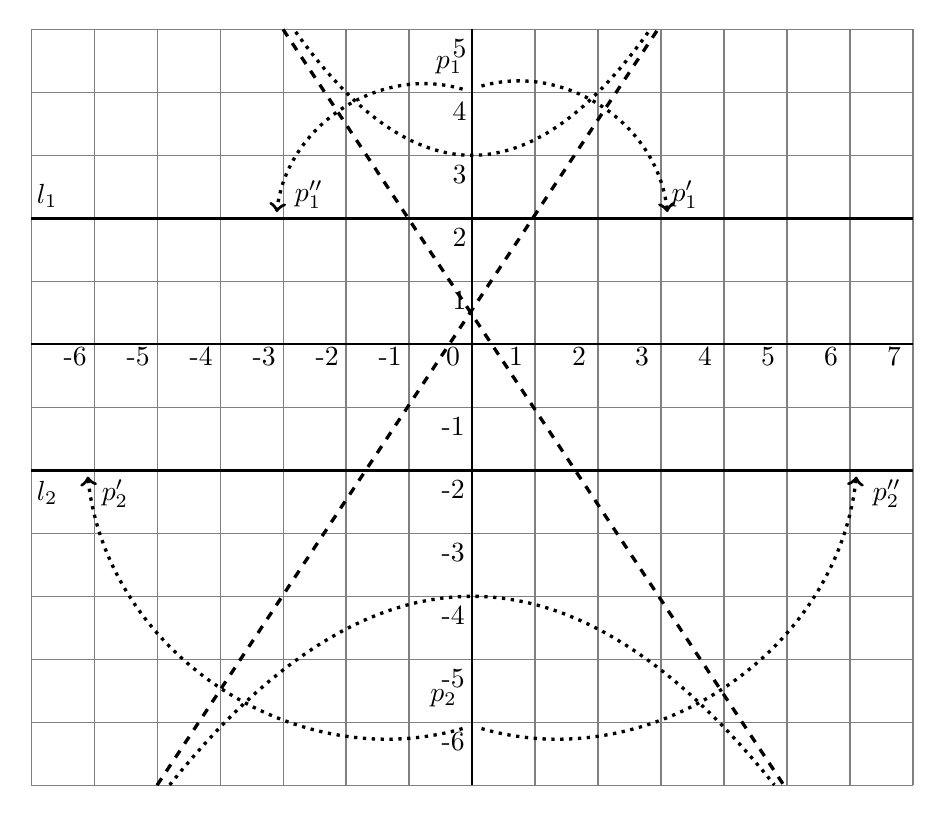
\begin{tikzpicture}[scale=.8]
\draw[step=10mm,white!50!black,thin] (-7,-7) grid (7,5);
\draw[thick] (-7,0) -- (7,0);
\draw[thick] (0,-7) -- (0,5);
\foreach \x in {-6,...,7}
  \node at (\x-.3,-.2) {\sm{\x}};
\foreach \y in {1,...,5}
  \node at (-.2,\y-.3) {\sm{\y}};
\foreach \y in {-6,...,-1}
  \node at (-.3,\y-.3) {\sm{\y}};
  
\coordinate (P1) at (0,4);
\coordinate (P2) at (0,-6);
\coordinate (P1P) at (3.1,2);
\coordinate (P2P) at (-6.12,-2);
\coordinate (P1PP) at (-3.1,2);
\coordinate (P2PP) at (6.12,-2);

\vertex{P1};
\vertex{P2};
\vertex{P1P};
\vertex{P2P};
\vertex{P1PP};
\vertex{P2PP};

\node[above left,yshift=3pt] at (P1) {$p_1$};
\node[above left,xshift=-2pt,yshift=2pt] at (P2) {$p_2$};
\node[above right,xshift=-2pt] at (P1P) {$p_1'$};
\node[below right,xshift=2pt] at (P2P) {$p_2'$};
\node[above right,xshift=3pt] at (P1PP) {$p_1''$};
\node[below right,xshift=2pt] at (P2PP) {$p_2''$};

\draw[very thick] (-7,2) -- node[very near start,above,xshift=-34pt] {$l_1$} (7,2);
\draw[very thick] (-7,-2) -- node[very near start,below,xshift=-34pt] {$l_2$} (7,-2);

\draw[domain=-4.8:4.8,samples=50,very thick,dotted] plot (\x,{-.13*\x*\x-4});
\draw[domain=-2.8:2.8,samples=50,very thick,dotted] plot (\x,{.25*\x*\x+3});

\draw[very thick,dashed] (-5,-7) -- (2.95,5);
\draw[very thick,dashed] (-3,5) -- (4.95,-7);

\draw[very thick,dotted,->,bend left=50] (.15,4.1) to (3.1,2.1);
\draw[very thick,dotted,->,bend right=50] (-.15,4.05) to (-3.1,2.1);

\draw[very thick,dotted,->,bend right=50] (.15,-6.1) to (6.1,-2.1);
\draw[very thick,dotted,->,bend left=50] (-.15,-6.1) to (-6.1,-2.1);

\end{tikzpicture}
\end{center}
\caption{Axioma $6$}\label{f.origami-axiom6}
\end{figure}

Para que un pliegue sitúe simultáneamente $p_1$ en $l_1$ y $p_2$ en $l_2$, debe ser una tangente común a las dos parábolas. Puede haber cero, una, dos o tres tangentes comunes (Figs.~\ref{f.two-para-1-zero}, \ref{f.two-para-1-one}, \ref{f.two-para-1-two}, \ref{f.two-para-1-three}).\index{Parabola!common tangents to two parabolas}

\begin{figure}[t]
\begin{minipage}{.45\textwidth}
\begin{center}
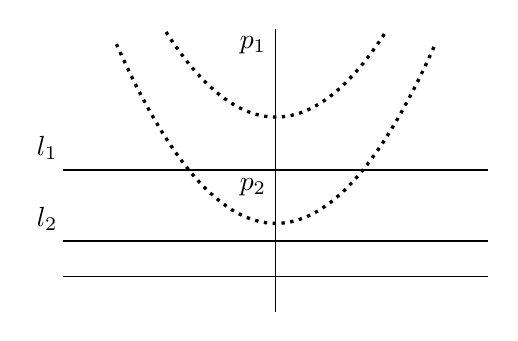
\begin{tikzpicture}[scale=.45]
\draw (-6,0) -- (6,0);
\draw (0,-1) -- (0,7);
\coordinate (P1) at (0,6);
\coordinate (P2) at (0,2);
\vertex{P1};
\vertex{P2};
\node[above left] at (P1) {$p_1$};
\node[above left] at (P2) {$p_2$};
\draw[thick] (-6,3) -- node[very near start,above,xshift=-25pt] {$l_1$} (6,3);
\draw[thick] (-6,1) -- node[very near start,above,xshift=-25pt] {$l_2$} (6,1);
\draw[domain=-3.1:3.1,samples=50,very thick,dotted] plot (\x,{.25*\x*\x+4.5});
\draw[domain=-4.5:4.5,samples=50,very thick,dotted] plot (\x,{.25*\x*\x+1.5});
\end{tikzpicture}
\caption{No hay tangentes comunes}\label{f.two-para-1-zero}
\end{center}
\end{minipage}
\hfill
\begin{minipage}{.45\textwidth}
\begin{center}
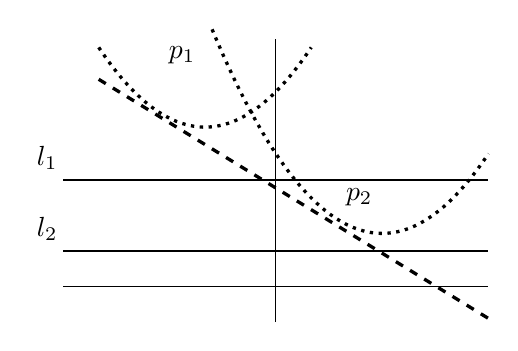
\begin{tikzpicture}[scale=.45]
\draw (-6,0) -- (6,0);
\draw (0,-1) -- (0,7);
\coordinate (P1) at (-2,6);
\coordinate (P2) at (3,2);
\vertex{P1};
\vertex{P2};
\node[above left] at (P1) {$p_1$};
\node[above left] at (P2) {$p_2$};
\draw[thick] (-6,3) -- node[very near start,above,xshift=-25pt] {$l_1$} (6,3);
\draw[thick] (-6,1) -- node[very near start,above,xshift=-25pt] {$l_2$} (6,1);
\draw[domain=-5:1,samples=50,very thick,dotted] plot (\x,{.25*(\x+2)*(\x+2)+4.5});
\draw[domain=-1.8:6,samples=50,very thick,dotted] plot (\x,{.25*(\x-3)*(\x-3)+1.5});
\draw[very thick,dashed] (-5,5.85) -- (6,-.9);
\end{tikzpicture}
\caption{Una tangente en común}\label{f.two-para-1-one}
\end{center}
\end{minipage}
%\end{figure}
%
%\begin{figure}[t]
\begin{minipage}{.45\textwidth}
\begin{center}
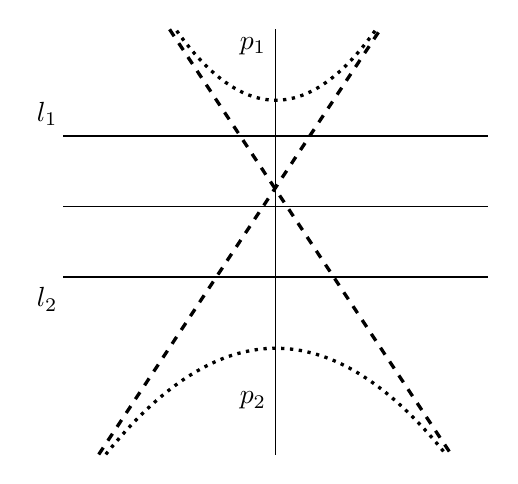
\begin{tikzpicture}[scale=.45]
\draw (-6,0) -- (6,0);
\draw (0,-7) -- (0,5);
\coordinate (P1) at (0,4);
\coordinate (P2) at (0,-6);
\vertex{P1};
\vertex{P2};
\node[above left] at (P1) {$p_1$};
\node[above left] at (P2) {$p_2$};
\draw[thick] (-6,2) -- node[very near start,above,xshift=-25pt] {$l_1$} (6,2);
\draw[thick] (-6,-2) -- node[very near start,below,xshift=-25pt] {$l_2$} (6,-2);
\draw[domain=-4.8:4.8,samples=50,very thick,dotted] plot (\x,{-.13*\x*\x-4});
\draw[domain=-2.8:2.8,samples=50,very thick,dotted] plot (\x,{.25*\x*\x+3});
\draw[very thick,dashed] (-5,-7) -- (2.95,5);
\draw[very thick,dashed] (-3,5) -- (4.95,-7);
\end{tikzpicture}
\caption{Dos tangentes en comunes}\label{f.two-para-1-two}
\end{center}
\end{minipage}
\hfill
\begin{minipage}{.45\textwidth}
\begin{center}
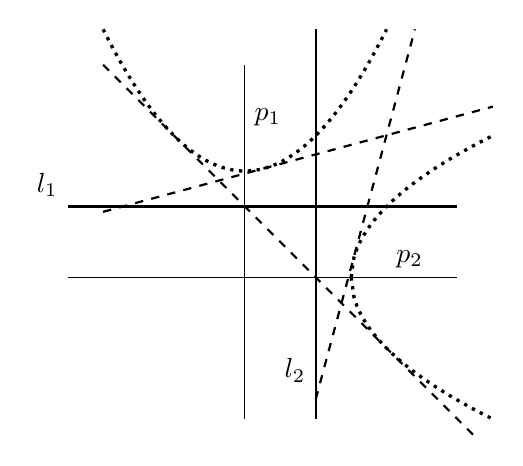
\begin{tikzpicture}[scale=.45]
\draw (-5,0) -- (6,0);
\draw (0,-4) -- (0,6);
\coordinate (P1) at (0,4);
\coordinate (P2) at (4,0);
\vertex{P1};
\vertex{P2};
\node[above right] at (P1) {$p_1$};
\node[above right] at (P2) {$p_2$};
\draw[thick] (-5,2) -- node[very near start,above,xshift=-25pt] {$l_1$} (6,2);
\draw[thick] (2,-4) -- node[very near start,left] {$l_2$} (2,7);
\draw[domain=-4:4,samples=50,very thick,dotted] plot (\x,{.25*\x*\x+3});
\draw[domain=3:7,samples=50,very thick,dotted] plot (\x,{sqrt(4*\x-12)});
\draw[domain=3:7,samples=50,very thick,dotted] plot (\x,{-sqrt(4*\x-12)});

\draw[thick,dashed,domain=-4:6.5] plot (\x,-\x+2);
\draw[thick,dashed,domain=-4:7] plot (\x,.27*\x+2.93);
\draw[thick,dashed,domain=2:4.8] plot (\x,3.73*\x-10.9);
\end{tikzpicture}
\caption{Tres tangentes en comunes}\label{f.two-para-1-three}
\end{center}
\end{minipage}
\end{figure}

La fórmula de una parábola arbitraria es bastante compleja, por lo que limitamos la presentación a las parábolas cuyo eje de simetría es el eje $x$ o $y$.

\subsection{Derivación de la ecuación de un pliegue}

Sea $(0,f)$ el foco de una parábola con directriz $y=d$. Definimos $p=f-d$, la longitud con signo del segmento entre el foco y la directriz\footnote{Hemos estado utilizando la notación $p_i$ para los puntos; el uso de $p$ aquí puede ser confuso, pero es la notación estándar. El nombre formal de $p$ es la mitad del \emph{latus rectum}.}. Si el vértice de la parábola está en el eje $x$ la ecuación de la parábola es $y=x^2/2p$. Para mover la parábola arriba o abajo del eje $y$ de forma que su vértice esté en $(0,h)$, se añade $h$ a la ecuación de la parábola (Fig.~\ref{f.elements-parabola}):
\[y=\frac{x^2}{2p}+h\,.\]

\begin{figure}[tb]
\begin{center}
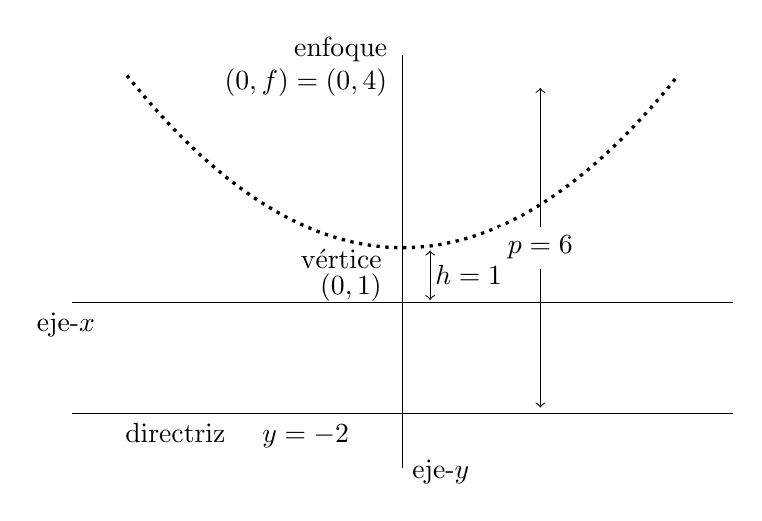
\begin{tikzpicture}[scale=.7]
\draw (-6,0) -- node[very near start,below,xshift=-32pt] {\textrm{eje}-$x$}(6,0);
\draw (0,-3) -- node[very near start,right,yshift=-20pt] {\textrm{eje}-$y$}(0,4.5);
\draw (-6,-2) -- node[near start,below] {\textrm{directriz} $\quad y=-2$} (6,-2);
\draw[domain=-5:5,samples=50,very thick,dotted] plot (\x,{\x*\x/8+1});
\coordinate (F) at (0,4);
\coordinate (V) at (0,1);
\coordinate (Y) at (0,-2);
\vertex{F};
\node[left,xshift=-2pt,yshift=0pt] at (F) {$(0,f)=(0,4)$}; \node[above left,xshift=-2pt,yshift=4pt] at (F) {\textrm{enfoque}};
\node[below left,xshift=-4,yshift=3pt] at (V) {\textrm{vértice}};
\node[below left,xshift=-4,yshift=-6pt] at (V) {$(0,1)$};
\draw[<->] (2.5,-1.9) -- node[fill=white] {$p=6$} +(0,5.8);
\draw[<->] (.5,.05) -- +(0,.9);
\node at (1.2,.5) {$h=1$} +(0,.9);
\end{tikzpicture}
\end{center}
\caption{Los elementos de la definición de una parábola}\label{f.elements-parabola}
\end{figure}
Definimos $a=2ph$ para que la ecuación de la parábola sea:
\begin{subeqnarray}
y&=&\frac{x^2}{2p}+\frac{a}{2p}\\
x^2-2py+a&=&0\,.\slabel{eq.eq-parabola}
\end{subeqnarray}
La ecuación de la parábola de la figura~\ref{f.elements-parabola} es $x^2-12y +12=0$.

Sustituimos la ecuación de una una línea \emph{arbitraria} $y=mx+b$ en la Ecuación~\ref{eq.eq-parabola} para obtener una ecuación de los puntos de intersección de la recta y la parábola:
\begin{eqnarray*}
x^2-2p(mx+b)+a&=&0\\
x^2+(-2mp)x+(-2pb+a)&=&0\,.
\end{eqnarray*}
La recta será tangente a la parábola si y sólo si esta ecuación cuadrática tiene \emph{exactamente una solución} si y sólo si su discriminante es cero:
\begin{subeqnarray}
(-2mp)^2\:-\:4\cdot 1\cdot (-2pb+a)=0\\
m^2p^2+2pb-a=0\,.\slabel{eq.disc}
\end{subeqnarray}
Se trata de una ecuación con variables $m,b$ para las tangentes a la parábola. Para obtener las tangentes comunes a ambas parábolas debemos resolver simultáneamente las ecuaciones de las dos parábolas.

\begin{example}\mbox{}

\noindent\textbf{Parábola 1:} Foco $(0,4)$, directriz $y=2$, vértice $(0,3)$.

\noindent{}$p=2$, $a=2\cdot 2\cdot 3=12$. La ecuación de la parábola es:
\[
x^2-4y +12=0\,.
\]
Sustituyendo $p$ y $a$ en la Ecuación~\ref{eq.disc} y simplificando da:
\[
m^2+b-3=0\,.
\]

\noindent\textbf{Parábola 2:} Foco $(0,-4)$, directriz $y=-2$, vértice $(0,-3)$.

\noindent{}$p=-2$, $a=2\cdot -2\cdot -3=12$. La ecuación de la parábola es:
\[
x^2+4y+12=0\,.
\]
Sustituyendo $p$ y $a$ en la Ecuación~\ref{eq.disc} y simplificando da:
\[
m^2-b-3=0\,.
\]
Las soluciones de las dos ecuaciones:
\begin{eqnarray*}
m^2+b-3&=&0\\
m^2-b-3&=&0
\end{eqnarray*}
son $m=\pm\sqrt{3}\approx \pm 1,73$ y $b=0$. Hay dos tangentes comunes:
\[
y=\sqrt{3}x\,,\quad y=-\sqrt{3}x\,.
\]
\end{example}

\begin{example}\mbox{}

\noindent\textbf{Parábola 1:}
Sin cambios.

\noindent\textbf{Parábola 2:} Enfoque $(0,-6)$, directriz $y=-2$, vértice $(0,-4)$.

\noindent{}$p=-4$, $a=2\cdot -4\cdot -4=32$. La ecuación de la parábola es:
\[
x^2+8y +32=0\,.
\]
Sustituyendo $p$ y $a$ en la Ecuación~\ref{eq.disc} y simplificando da:
\[
2m^2-b-4=0\,.
\]
Las soluciones de las dos ecuaciones:
\begin{eqnarray*}
m^2+b-3&=&0\\
2m^2-b-4&=&0
\end{eqnarray*}
son $m=\pm\sqrt{\displaystyle\frac{7}{3}}\approx \pm 1.53$ y $b=\displaystyle\frac{2}{3}$. Hay dos tangentes comunes:
\[
y=\sqrt{\frac{7}{3}}x+\frac{2}{3}\,,\quad y=-\sqrt{\frac{7}{3}}x+\frac{2}{3}\,.
\]
\end{example}

%%%%%%%%%%%%%%%%%%%%%%%%%%%%%%%%%%%%%%%%%%%%%%%%%%%%%%%%%%%%%%%%

\begin{example}\mbox{}

\noindent Definamos ahora una parábola cuyo eje de simetría es el eje $x$.

\noindent\textbf{Parábola 1:} Sin cambios. 

\noindent\textbf{Parábola 2:} Foco $(4,0)$, directriz $x=2$, vértice $(3,0)$.

\noindent{}$p=2$, $a=2\cdot 2\cdot 3=12$. La ecuación de la parábola es:
\begin{align}
y^2-4x+12 = 0\,.\label{eq.x-symmetry-parabola}
\end{align}
Esta es una ecuación con $x$ y $y^2$ en lugar de $x^2$ e $y$, por lo que la Ecuación~\ref{eq.disc} no se puede utilizar y debemos realizar la derivación de nuevo.

Sustituir la ecuación de una recta en la Ecuación~\ref{eq.x-symmetry-parabola}:
\begin{eqnarray*}
(mx+b)^2-4x+12&=&0\\
m^2x^2+(2mb-4)x+(b^2+12)&=&0\,.
\end{eqnarray*}
Igualamos el discriminante a cero y simplificamos:
\begin{eqnarray*}
(2mb-4)^2\:-\:4m^2(b^2+12)&=&0\\
-3m^2-mb+1&=&0\,.
\end{eqnarray*}
Si intentamos resolver las dos ecuaciones:
\begin{eqnarray*}
m^2+b-3&=&0\\
-3m^2-mb+1&=&0\,,
\end{eqnarray*}
obtenemos una ecuación \emph{cúbica} con variable $m$:\index{Parabola!cubic equation for the common tangents}
\begin{align}
m^3-3m^2-3m+1=0\,.\label{eq.cubic}
\end{align}
Como una ecuación cúbica tiene como mínimo una y como máximo tres soluciones reales, puede haber una, dos o tres tangentes comunes.

La fórmula para resolver ecuaciones cúbicas generales es bastante complicada, así que he utilizado una calculadora de Internet y he obtenido las tres soluciones:
\[m=3.73,\:m=-1,\:m=0.27\,.\]
A partir de la forma de la Ecuación~\ref {eq.cubic} podríamos suponer que $m=1$ o $m=-1$ es una solución:
\begin{eqnarray*}
1^3-3\cdot 1^2-3\cdot 1+1&=&-4\\
(-1)^3-3\cdot (-1)^2-3\cdot(-1)+1&=&0\,.
\end{eqnarray*}
Dividimos Ecuación~\ref{eq.cubic} por $m-(-1)=m+1$ para obtener la ecuación cuadrática $m^2-4m+1$ cuyas raíces son las otras dos soluciones de la ecuación cúbica $m=2\pm\sqrt{3}\approx 3.73, 0.27$.
\end{example}

%%%%%%%%%%%%%%%%%%%%%%%%%%%%%%%%%%%%%%%%%%%%%%%%%%%%%%%%%%%%%%%%

\subsection{Derivación de las ecuaciones de las reflexiones}

Derivamos la posición de la reflexión $p_1'=(x_1',y_1')$ de $p_1=(x_1,y_1)$ alrededor de una recta tangente $l_t$ cuya ecuación es $y=m_tx+b_t$. Primero, hallamos la recta $l_p$ de ecuación $y=m_px+b_p$ que es perpendicular a $l_t$ y pasa por $p_1$:
\begin{eqnarray*}
y&=&-\frac{1}{m_t}x+b_p\\
y_1&=&-\frac{1}{m_t}x_1+b_p\\
y&=&\frac{-x}{m_t}+\left(y_1+\frac{x_1}{m_t}\right)\,.
\end{eqnarray*}
A continuación hallamos la intersección $p_t=(x_t,y_t)$ de $l_t$ y $l_p$:
\begin{eqnarray*}
m_tx_t+b_t&=&\frac{-x_t}{m_t}+\left(y_1+\frac{x_1}{m_t}\right)\\
x_t&=&\frac{\left(y_1+\displaystyle\frac{x_1}{m_t}-b_t\right)}{\left(m_t+\displaystyle\frac{1}{m_t}\right)}\\
y_t&=&m_tx_t+b_t\,.
\end{eqnarray*}
$p_t$ es el punto medio entre $p_1$ y $p_1'$:
\[
\begin{array}{rcl@{\hspace{3ex}}rcl}
x_t&=&\displaystyle\frac{x_1+x_1'}{2}\,, &x_1'&=&2x_t-x_1\,,\\
y_t&=&\displaystyle\frac{y_1+y_1'}{2}\,,& y_1'&=&2y_t-y_1\,.
\end{array}
\]
\begin{example}
Sea $l_t$ $y=\sqrt{3}x+0$ y sea $p_1=(0,4)$:
\begin{eqnarray*}
x_t&=&\frac{\left(4+\displaystyle\frac{0}{\sqrt{3}}-0\right)}{\left(\sqrt{3}+\displaystyle\frac{1}{\sqrt{3}}\right)}=\sqrt{3}\\
y_t&=&\sqrt{3}\sqrt{3}+0=3\\
x_1'&=&2x_t-x_1=2\sqrt{3}\approx 3.46\\
y_1'&=&2y_t-y_1= 2\,.
\end{eqnarray*}
\end{example}

%%%%%%%%%%%%%%%%%%%%%%%%%%%%%%%%%%%%%%%%%%%%%%%%%%%%%%%%%%%%%%%%

\subsection{Tangentes a una parábola}\label{s.parabola}

Queremos demostrar que los pliegues del axioma 6 son tangentes a las parábolas.
La figura~\ref{f.parabola-locus} muestra cinco puntos
$p_i$, $i=1,\ldots,5$, cada punto $p_i$ a una distancia $a_i$ tanto del foco como de la directriz. Se trazan rectas perpendiculares desde $p_i$ a la directriz y se denotan las intersecciones de estas rectas con la directriz por $p_i'$. Por Axioma~$2$ existen pliegues $l_i$ que pasan por $p_i$ y sitúan $p$ en la directriz. Los puntos $p_i'$ son las reflexiones de $p$ alrededor de los pliegues. La figura muestra el pliegue $l_1$ que atraviesa $p_1$ y la reflexión $p_1'$.

\begin{figure}[t]
\begin{center}
\begin{tikzpicture}[scale=.8]
\draw (-6,0) -- node[very near start,below,xshift=-32pt] {eje-$x$} (6,0);
\draw (0,-3) -- node[very near start,right,yshift=-15pt] {eje-$y$} (0,4.5);
\draw[thick] (-6,-2) -- node[near end,below] {directriz $\quad y=-f$} (6,-2);
\draw[domain=-6:6,samples=50,very thick,dotted] plot (\x,{\x*\x/8});
\coordinate (F) at (0,2);
\vertex{F};
\node[above left,xshift=-2pt,yshift=15pt] at (F) {$(0,f)$};
\node[above left,xshift=-5pt,yshift=26pt] at (F) {focus}; \node[above right] at (F) {$p$};
\coordinate (vertex) at (0,0);
\vertex{vertex};
\node[below right] at (vertex) {$p_2$};
\coordinate (FP) at (-5,-2);
\node[below] at (FP) {$p_1'$};
\coordinate (F1) at (2,.5);
\vertex{F1};
\node[below right] at (F1) {$p_3$};
\coordinate (F2) at (3,1.125);
\vertex{F2};
\node[below right] at (F2) {$p_4$};
\coordinate (F3) at (5,3.125);
\vertex{F3};
\node[below right] at (F3) {$p_5$};
\coordinate (F4) at (-5,3.125);
\vertex{F4};
\node[above right] at (F4) {$p_1$};
\draw (F) -- node[left] {$a_2$} (0,0) -- node[left] {$a_2$} (0,-2);
\draw (F) -- node[near end,left] {$a_3$} (F1) -- node[left] {$a_3$} (2,-2);
\draw (F) -- node[near end,above] {$a_4$} (F2) -- node[left] {$a_4$} (3,-2);
\draw (F) -- node[above] {$a_5$} (F3) -- node[left] {$a_5$} (5,-2);
\draw (F) -- node[above] {$a_1$} (F4) -- node[left] {$a_1$} (FP);
\draw[very thick,dashed] ($(F4)!-.4!(-2.5,0)$) -- node[near end,right,xshift=2pt] {$l_1$} ($(F4)!1.8!(-2.5,0)$);
\draw (0,-2) rectangle +(9pt,9pt);
\draw (2,-2) rectangle +(9pt,9pt);
\draw (3,-2) rectangle +(9pt,9pt);
\draw (5,-2) rectangle +(9pt,9pt);
\draw (-5,-2) rectangle +(9pt,9pt);
\end{tikzpicture}
\end{center}
\caption{La tangente como lugar geométrico}\label{f.parabola-locus}
\end{figure}

\begin{figure}[thb]
\begin{center}
\begin{tikzpicture}[scale=.8]
\draw[thick] (-6,-2) -- node[near end, below] {$d$} (6,-2);
\draw[domain=-5.5:5.5,samples=50,very thick,dotted] plot (\x,{\x*\x/8});
\coordinate (F) at (0,2);
\vertex{F};
\node[above right] at (F) {$p$};
\coordinate (FP) at (-3,-2);
\node[below] at (FP) {$p'$};
\coordinate (F4) at (-3,1.125);
\vertex{F4};
\node[above right] at (F4) {$r$};
\coordinate (F5) at (-5,2.775);
\vertex{F5};
\node[left,yshift=-4pt] at (F5) {$q$};
\coordinate (F5p) at (-5,-2);
\node[below] at (F5p) {$p''$};
\draw (F) -- node[above] {$b$} (F4) -- node[left] {$b$} (FP);
\draw (F) -- node[above] {$c$} (F5);
\draw (F5) -- node[left] {$e$} (F5p);
\draw[thick,dashed,name path=fold] ($(F4)+(140:4)$) -- (F4) -- node[below,xshift=3pt,yshift=-4pt] {$l$} ($(F4)+(-40:5.3)$);
\draw (FP) rectangle +(10pt,10pt);
\draw (F5p) rectangle +(10pt,10pt);
\draw (F5) -- (FP);
\draw[name path=base] (F) -- (FP);
\path [name intersections = {of = base and fold, by = {G}}];
\node[below,yshift=-4pt] at (G) {$s$};
\draw[rotate=140] (G) rectangle +(10pt,10pt);
\path (FP) -- node[left] {$c$} (F5);
\path (F) -- node[below] {$a$} (G) -- node[below] {$a$} (FP);
\end{tikzpicture}
\end{center}
\caption{La demostración de que el pliegue es una tangente}\label{f.tangent-proof}
\end{figure}

\begin{theorem}\label{thm.parabola-tangents}
Los pliegues del axioma~$6$ son las tangentes a las parábolas que son los lugares geométricos de los puntos equidistantes a los puntos $p_1,p_2$ y $l_l,l_2$, respectivamente.
\end{theorem}
\begin{proof}
En la figura~\ref{f.tangent-proof}, el foco es $p$ y la directriz es $d$. $p'$ es un punto de la directriz y $l$ es el pliegue que refleja $p$ en $p'$. Sea $s$ la intersección de $\overline{pp'}$ y $l$. Entonces $\overline{ps}=\overline{p's}=a$ y $l\perp \overline{pp'}$ ya que $l$ es la mediatriz de $\overline{pp'}$.

Sea $r$ la intersección de la recta perpendicular a $d$ que pasa por $p'$ y el pliegue $l$. Entonces $\triangle psr\cong \triangle p'sr$ por lado-ángulo-lado. Se deduce que 
$\overline{pr}=\overline{p'r}=b$ por lo que $r$ es un punto de la parábola. Elegimos un punto $p''$ sobre la directriz que sea distinto de $p'$ y suponemos que el pliegue $l$ también refleja $p$ sobre $p''$. Sea $q$ la intersección de la perpendicular a $d$ que pasa por $p''$ y el pliegue $l$. $\triangle psq\cong \triangle p'sq$ por lo que $\overline{pq}=\overline{p'q}=c$. Denotemos $\overline{qp''}=e$. Si $q$ es un punto de la parábola entonces $e=\overline{qp''}=\overline{qp}=c$, pero $c$ es la hipotenusa del triángulo rectángulo $\triangle qp''p'$ y no es posible que la hipotenusa sea igual a uno de los otros lados del triángulo rectángulo. Por lo tanto el pliegue $l$ sólo tiene una intersección con la parábola y debe ser una tangente.
\end{proof}

%%%%%%%%%%%%%%%%%%%%%%%%%%%%%%%%%%%%%%%%%%%%%%%%%%%%%%%%%%%%%%%%

\section{Axioma 7}\label{s.ax7}

\index{Origami!axiom 7}
\begin{axiom}
Dado un punto $p_1$ y dos rectas $l_1$ y $l_2$, existe un pliegue $l$ que sitúa $p_1$ sobre $l_1$ y es perpendicular a $l_2$ (Fig.~\ref{f.origami-axiom7}).
\end{axiom}

El pliegue es el lugar geométrico de todos los puntos de la recta perpendicular a $l_2$ y equidistante de $p_1$ y $p_1'$, la reflexión de $p_1$ sobre $l_1$.

\smallskip

\noindent\textbf{Derivación de la ecuación del pliegue:}
Sea $p_1=(x_1,y_1)$, sea $l_1$ $y = m_1x + b_1$ y sea $l_2$ $y=m_2x+b_2$. Sea $l_p$ la recta que contiene a $\overline{p_1p_1'}$. Como $l\perp l_2,l_p\perp l$, resulta que $l_p\parallel l_2$ y la ecuación de $l_p$ es $y=m_2x+b_p$.

\begin{figure}[t]
\begin{center}
\begin{tikzpicture}[scale=.8]
\draw[step=10mm,white!50!black,thin] (-1,-1) grid (9,8);
\draw[thick] (-1,0) -- (9,0);
\draw[thick] (0,-1) -- (0,8);
\foreach \x in {0,...,9}
  \node at (\x-.2,-.2) {\sm{\x}};
\foreach \y in {1,...,8}
  \node at (-.2,\y-.3) {\sm{\y}};
  
\coordinate (P1) at (5,3);
\node[below left] at (P1) {$p_1$};
\vertex{P1};

\coordinate (P1P) at (2.75,5.25);
\node[left,xshift=-4pt] at (P1P) {$p_1'$};
\vertex{P1P};

\draw (1,0) -- node[very near start,right,xshift=2pt] {$l_1$} (3,6);
\draw[name path=l2] (8,3) -- node[very near start,right,xshift=-2pt,yshift=6pt] {$l_2$} (5,6);

\draw ($(1,0)!-.16!(3,6)$) -- ($(1,0)!1.33!(3,6)$);

\draw ($(8,3)!-.33!(5,6)$) -- ($(8,3)!1.66!(5,6)$);

\draw ($(P1)!-.4!(P1P)$) -- node[very near start,below,yshift=-4pt] {$l_p$} ($(P1)!1.5!(P1P)$);

\draw[very thick,dashed,name path=fold] (-1,-.75) -- node[very near end,above,xshift=4pt,yshift=6pt] {$l$} (7.75,8);

\coordinate (mid) at ($(P1)!.5!(P1P)$);
\node[below,yshift=-8pt] at (mid) {$p_m$};

\path [name intersections = {of = fold and l2, by = {perp}}];
\draw[rotate=-45] (mid) rectangle +(8pt,8pt);
\draw[rotate=-45] (perp) rectangle +(8pt,8pt);


\draw[very thick,dotted,->,bend right=50] (5.05,3.1) to (2.85,5.24);
\end{tikzpicture}
\end{center}
\caption{Axioma $7$}\label{f.origami-axiom7}
\end{figure}

$l_p$ pasa por $p_1$ por lo que $y_1=m_2x_1+b_p$ y su ecuación es $y=m_2x+(y_1-m_2x_1)$. La reflexión $p_1'=(x_1',y_1')$ es la intersección de $l_1$ y $l_p$:
\begin{eqnarray*}
m_1x_1'+b_1&=&m_2x_1'+(y_1-m_2x_1)\\
x_1'&=&\frac{y_1-m_2x_1-b_1}{m_1-m_2}\\
y_1'&=&m_1x_1'+b_1\,.
\end{eqnarray*}
La ecuación del punto medio $p_m=(x_m,y_m)$ de $l_p$ es:
\[
(x_m,y_m)=\left(\frac{x_1+x_1'}{2},\frac{y_1+y_1'}{2}\right)\,.
\]
$l\perp l_2$ y pasa por $p_m$ por lo que su ecuación es:
\[
y=-\frac{1}{m_2}x+b_m,
\]
donde $b_m$ puede calcularse a partir de $y=-\displaystyle\frac{1}{m_2}x+b_m$:
\[b_m=y_m+\frac{x_m}{m_2}\,.\]
Por lo tanto, la ecuación del pliegue $l$ es:
\[
y=-\frac{1}{m_2}x+\left(y_m+\displaystyle\frac{x_m}{m_2}\right)\,.
\]
\begin{example}
Sea $p_1=(5,3)$, $l_1$ $y=3x-3$ y $l_2$ $y=-x+11$. Entonces:
\begin{eqnarray*}
x_1'&=&\frac{3-(-1)\cdot 5-(-3)}{3-(-1)}=\frac{11}{4}\\
y_1'&=&3\cdot \frac{11}{4} + (-3)=\frac{21}{4}\\
p_m&=&\left(\frac{5+\displaystyle\frac{11}{4}}{2},\frac{3+\displaystyle\frac{21}{4}}{2}\right)=\left(\frac{31}{8},\frac{33}{8}\right)\,.
\end{eqnarray*}
La ecuación del pliegue $l$ es:
\[
y=-\frac{1}{-1}\cdot x+\left(\frac{33}{8}+\frac{\displaystyle\frac{31}{8}}{-1}\right)=x+\frac{1}{4}\,.
\]
\end{example}

\subsection*{¿Cuál es la sorpresa?}

El origami, el arte de plegar papel, se practica desde hace cientos de años, por lo que sorprende que la formalización matemática se remonte sólo al siglo XX. Sorprende aún más que exista una axiomatización del plegado de papel. Las matemáticas del origami son una excelente manera de aprender geometría analítica, propiedades de las parábolas y el concepto de lugar geométrico.



\subsection*{Fuentes}

Los axiomas del origami se presentan en \cite{wiki:hh-axioms}. Lang \cite{lang} ofrece descripciones de construcciones de origami. 
\cite[Capítulo~10]{martin} contiene la teoría detallada de las matemáticas del origami, incluyendo la demostración de que dos parábolas pueden tener cero, una, dos o tres tangentes comunes. La demostración de Teorema~\ref{thm.parabola-tangents} me fue mostrada por Oriah Ben-Lulu. He encontrado que el software geométrico como Geogebra es útil para entender la relación entre la geometría y el álgebra de los axiomas.

Una presentación clara de las ecuaciones cúbicas se puede encontrar en \cite[Capítulos~1,\ 2]{jorg}.
